\chapter{Implementierung}
\label{chap:implementation}

In diesem Kapitel wird erläutert, wie \name und alle in 
Kapitel~\ref{chap:concept} beschriebenen Komponenten implementiert wurden.\\
Zusätzlich wird beschrieben, wie \name in das \ac{IRL} als
Demonstrator integriert wurde.

\section{Datenbank}
\label{sec:implementation:db}

Für die Datenbank wurde ein relationales Datenbankmanagementsystem
gesucht, welches unter einer freien Lizenz steht, auf möglichst vielen
Betriebssystemen läuft, aktiv weiterentwickelt wird und sich auf
großen Produktivsystemen bewährt hat.\\
Näher betrachtet wurden dabei "`MySQL"' bzw. der Fork "`MariaDB"' und
"`PostgreSQL"'.\\
Entschieden wurde sich für das objektrelationale
Datenbankmanagementsystem PostgreSQL in Version 9.2.4, da dieses System
zusätzlich zu den oben genannten Kriterien größtenteils den
SQL-Standard 2008 implementiert und standardmäßig mehr Daten in
einer Tabelle
speichern kann, was sich zur Erstellung einer Produktdatenbank mit sehr vielen 
Produkten gut eignet.
PostgreSQL wird seit 1995 aktiv weiterentwickelt
\citeweb{postgresql:about, wiki:rdbms}.\\
Das Datenbankmodell, das in \name benutzt wurde, befindet sich im
Anhang~\ref{appendix:db} und wird auch in der technischen
Dokumentation (siehe Abschnitt~\ref{sec:implementation:docu}) näher beschrieben.
Das stark vereinfachte Datenbankmodell in Abbildung~\ref{img:mini_models} 
(abgeleitet von dem Modell im Anhang) soll dabei einen 
Überblick über die wichtigsten Tabellen und Relationen bieten.

\begin{figure}[ht]
  \centering
  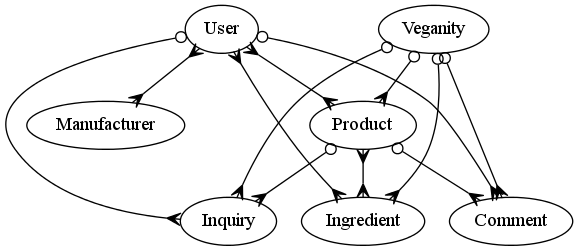
\includegraphics[scale=0.6]{misc/mini_models.png}
  \caption{Stark vereinfachtes Datenbankmodell}
  \label{img:mini_models}
\end{figure}

Zu sehen sind die wichtigsten Tabellen "`User"', "`Veganity"', 
"`Manufacturer"', "`Product"', "`Inquiry"', "`Ingredient"' und "`Comment"'. Die 
Beziehung untereinander wird durch die Pfeilarten symbolisiert.
So hat jedes Produkt, jede Produktanfrage, Zutat und jeder Kommentar eine 
Veganität. Weiterhin kann ein*e Nutzer*in viele Kommentare, Produktanfragen, 
Hersteller*innen, Produkte und Zutaten erstellen, aber nur die 
Hersteller*innen, Zutaten und Produkte können von vielen Nutzer*innen geändert 
werden. Zudem enthält ein Produkt viele Produktanfragen, Kommentare und Zutaten 
und jede Zutat wiederum viele Produkte, was ausführlicher in 
Abschnitt~\ref{sec:implementation:ingredients} beschrieben.

\section{Mobile App}
\label{sec:implementation:app}

Zusätzlich zu einer Webanwendung sollten für möglichst alle mobilen
Betriebssysteme je eine \ac{App} erstellt werden, da im Alltag
eher mobile Begleiter wie Smartphones anstelle von Desktop-PCs genutzt werden
und somit auch die Hardwarekomponenten der mobilen Geräte benutzt werden
können um beispielsweise einen Barcode scannen zu können.\\
Um nicht für jedes mobile Betriebssystem eine eigene native \ac{App} in
unterschiedlichen Sprachen wie Java und Objective-C erstellen zu
müssen, wurde sich für die freie Lösung PhoneGap in Version 3.0.0
entschieden, die bereits in
Abschnitt~\ref{sec:phonegap} näher beschrieben wurde.\\
Obwohl mit PhoneGap plattformübergreifende mobile Apps möglich sind,
wurde der Fokus auf das freie Betriebssystem Android ab Version 4.1
gelegt, da dieses den
größten Marktanteil besitzt \citeweb{wiki:mobile}.

\section{Webanwendung}
\label{sec:implementation:web}

Für die Webanwendung wurde ein freies, plattformübergreifendes
Webframework auf Basis der
Sprachen PHP, Python oder Ruby gesucht, welches aktiv weiterentwickelt 
wird.
Zusätzlich sollte das
Muster \ac{MVC}
benutzt werden und
sich ebenfalls wie die Datenbank auf großen Produktivsystemen bewährt
haben.\\
Näher betrachtet wurden dabei "`Zend Framework"', "`Django"' und
"`\ac{RoR}"'.\\
Die Wahl fiel dabei auf
\ac{RoR} in Version 4.0.0, welches die oben genannten Kriterien 
erfüllt und
leicht durch RubyGems, d.\,h. Pakete, erweiterbar ist.
\ac{RoR} wird seit 2004 aktiv weiterentwickelt \citeweb{rails,
wiki:webframework}.

Das in Abschnitt~\ref{sec:concept:layout} beschriebene Layout wurde mit Hilfe 
von 
"`Bootstrap"', einer Sammlung von Hilfsmitteln zur Gestaltung einer Website, 
realisiert, dass sich gut in \ac{RoR} integriert, ein responsive Webdesign 
(vgl. Abschnitt~\ref{sec:concept:webapp}) umsetzt und schon auf vielen großen
Plattformen wie Twitter und GitHub als Bedienoberfläche eingesetzt wird.

\subsection{Registrierung}
\label{sec:implementation:users}

Die Registrierung der Nutzer*innen erfolgt wie in 
Abschnitt~\ref{sec:concept:users} beschrieben mit Hilfe von 
Authentifizierungs-Anbieter*innen, in diesem Fall mit Google, Facebook, Twitter 
und GitHub über das in Abschnitt~\ref{sec:oauth} beschriebene Verfahren OAuth.
Bei der Registrierung werden nach dem Erlauben von Datenfreigaben auf der Seite 
der Anbieter*innen die Daten zu \name geleitet und in der Tabelle \code{users} 
in der Datenbank gespeichert.
Zusätzlich wird eine E-Mail mit einer Begrüßung und einem Link an die 
E-Mailadresse versendet, die bei der*dem jeweiligen Anbieter*in angegeben wurde, 
um die E-Mailadresse zu verifizieren.
Dazu wird ein zufälliger Wert generiert und in der Datenbank in der Tabelle 
\code{emailhashes} gespeichert. Mit Hilfe des Keccak-Algorithmus \cite{bdpv11} 
wird daraus ein sogenannter Hash generiert, der in der E-Mail an einen Link 
angehängt wird. Wird der Link aufgerufen, wird der angehängte Hash mit dem Wert 
in der Datenbank verglichen. Sind die beiden Werte gleich und nicht länger als 
drei Tage in der Datenbank vorhanden, gilt die E-Mailadresse als validiert und 
wird mit Punkten "`belohnt"' (vgl. 
Abschnitt~\ref{sec:implementation:gamification}).

\subsection{Gamifizierung}
\label{sec:implementation:gamification}

Wie in Abschnitt~\ref{sec:concept:gamification} beschrieben, wird die 
sogenannte Gamifizierung verwendet, um bei den Nutzer*innen ein Anreiz zu 
schaffen, etwas zu leisten. Die dort beschriebenen Punkte und Befugnisse werden 
im Folgenden konkretisiert.

Punkte können durch verschiedene Aktionen "`verdient"' werden, wie in
Tabelle~\ref{table:points} dargestellt ist. Dabei spielt es bei manchen 
Aktionen auch eine Rolle, welche Rechte vorhanden sind, beispielsweise 
kann ein Kommentar nur mit einem Befugnis "`1"' erstellt werden.

\begin{table}[ht]
	\rowcolors{2}{gray!25}{white}
	\begin{tabular}{c|c|l}
		\rowcolor{gray!50}
		Punkte & Rechte & Beschreibung\\
			\hline
		5 & 1 & Neuer Kommentar\\
		10 & 0 & Vollständig ausgefülltes Produkt\\
		10 & 2 & Neue Produktanfrage\\
		10 & 0 & Validierung der E-Mailadresse\\
		25 & 0 & Neues Produkt\\
		40 & 2 & Einfügen der Antwort auf eine Produktanfrage\\
	\end{tabular}
	\caption{Punkte, die durch eine bestimmte Aktion
	"`verdient"' werden können, wobei manche Aktionen nur mit höheren 
Rechten ausgeführt werden können.}
	\label{table:points}
\end{table}

Die Rechte wiederum können teilweise durch Punkte verdient werden, was in 
Tabelle~\ref{table:permissions} ersichtlich wird.
\begin{table}[ht]
	\rowcolors{2}{gray!25}{white}
	\begin{tabular}{c|c|l}
		\rowcolor{gray!50}
		Rechte & Mindestpunktzahl & Beschreibung\\
			\hline
			0 & 0 & Standard Rechte (Produkt, Hersteller, usw. 
anlegen)\\
			1 & 250 & Kommentar schreiben\\
			2 & 500 & Produktanfrage schreiben/einfügen\\
			2 & 500 & Quelle zu Produkt hinzufügen\\
			3 & 1000 & Zutat manuell erstellen und verändern\\
			5 & - & Einträge löschen\\
			10 & - & Administrator*in
	\end{tabular}
	\caption{Befugnisse, die je nach Mindestpunktzahl erreicht 
werden
	können. Einige Rechte können nur von den Administrator*innen
	vergeben werden (mit "`-"' gekennzeichnet).}
	\label{table:permissions}
\end{table}
Je nach Mindestpunktanzahl können dabei gewisse Rechte bzw. Befugnisse
freigeschaltet werden, um so einerseits wieder einen Anreiz zu
schaffen, mehr Daten in die Datenbank einzugeben und andererseits
einem Missbrauch vorzubeugen.
Einige Befugnisse können dabei
nicht durch Punkte freigeschaltet werden (gekennzeichnet mit "`-"' in der 
Tabelle), können allerdings von den
Administrator*innen vergeben werden.\\
Der*Die erste Administrator*in muss dabei durch eine Modifikation der Datenbank 
festgelegt werden, was in der technischen Dokumentation (siehe 
Abschnitt~\ref{sec:implementation:docu}) beschrieben ist.

Um einen Anreiz zu schaffen, ein Produkt möglichst vollständig auszufüllen, 
wird unter jedem Produkt durch eine Fortschrittsanzeige visuell die 
Vollständigkeit angezeigt, was in Abbildung~\ref{img:integrity} dargestellt ist.

\begin{figure}[ht]
  \centering
  
\includegraphics[scale=0.45]{pics/integrity.png}
  \caption{Vollständigkeitsanzeige, die unter jedem Produkt angezeigt wird}
  \label{img:integrity}
\end{figure}

Dieser Wert wird berechnet durch neun Indikatoren, die bei einem Produkt 
angegeben werden müssen: 
Barcode bzw. \ac{GTIN}, Name, Beschreibung, Zutaten, 
Kategorie, Verpackungsmaterial, Verpackungsgröße, Herkunftsland und Marke.
Alle anderen Angaben sind optional, da sie nicht bei jedem Produkt 
vorliegen.

Eine Bestenliste, welche die Nutzer*innen mit Avatar, Spitzname und
Punktanzahl auflistet, soll für einen kleinen Wettbewerb untereinander
sorgen, wobei dadurch wieder mehr Produkte eingetragen bzw. Einträge
vervollständigt werden sollen.
Dabei werden auf der Nutzer*innenübersicht alle Nutzer*innen nach Punkten und 
danach alphabetisch nach Spitzname sortiert, wobei sich die Besten in der Liste 
ganz oben befinden. Dies ist in Abbildung~\ref{img:leaderboard} in einem 
Ausschnitt zu sehen.

\begin{figure}[ht]
  \centering
  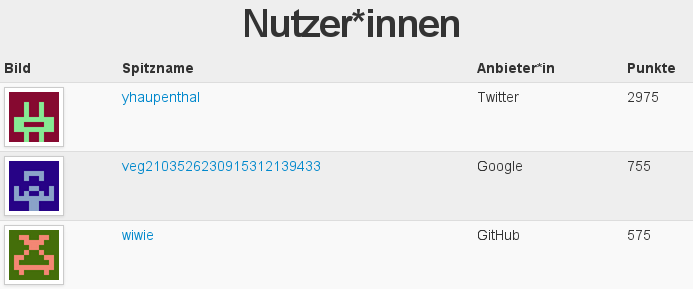
\includegraphics[scale=0.5]{pics/leaderboard.png}
  \caption{Bestenliste, mit den Nutzer*innen nach Punkten absteigend sortiert}
  \label{img:leaderboard}
\end{figure}

\subsection{Extraktion von Zutateninformationen und -veganitäten}
\label{sec:implementation:ingredients}

Bei der Produkterstellung können Zutaten angegeben werden, die automatisch 
erstellt werden und zur Veganitätsbestimmung des Produktes dienen. Dies wird in 
Abbildung~\ref{img:new_product} verdeutlicht, wobei neben den Pflichtangaben 
(siehe Abschnitt~\ref{sec:concept:product}) optionale Angaben möglich sind.

\begin{figure}[ht]
  \centering
  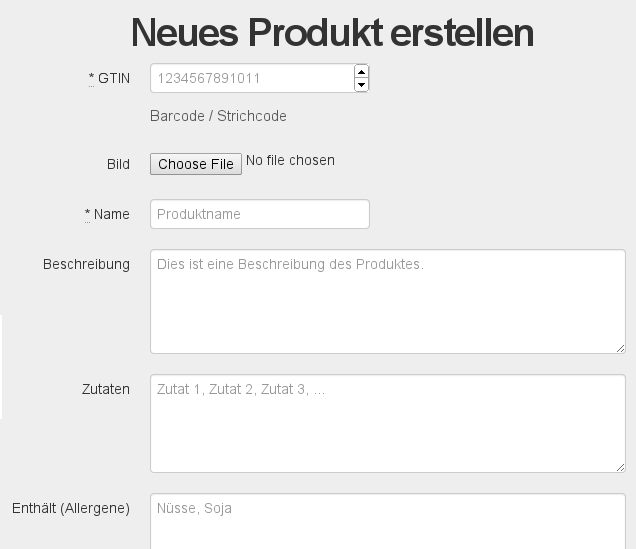
\includegraphics[scale=0.5]{pics/new_product.png}
  \caption{Anlegung eines neuen Produktes, u.\,a. mit einer Möglichkeit zur 
manuellen Eingabe einer Zutatenliste}
  \label{img:new_product}
\end{figure}

Zur Erstellung der Zutaten werden die Zutatenliste mit Hilfe von regulären 
Ausdrücken geparst und Klassennamen wie "`Emulgator"' -- welche in den Tabellen
\code{classnames} und \code{classnames\_synonyms} gespeichert sind --
herausgefiltert um so nur noch die eigentlichen Zutaten zu erhalten.
Die Zutaten können dabei auch durch die Zutatensynonyme, die bei einer Zutat 
angegeben werden können, erkannt werden. Wurden bei diesem Vorgang Zutaten 
erstellt, die Rechtschreibfehler enthalten oder Zutaten darstellen, die aus 
anderen Zutaten zusammengesetzt sind wie z.\,B. "`Tofu"' oder "`Teig"' können 
diese durch die Administrator*innen bzw. durch jeweilige Rechte "`versteckt"' 
werden und tauchen daraufhin in keinen Übersichten oder 
Zutatenlisten mehr auf. Dieses Verstecken bietet im Gegensatz zur Löschung 
den Vorteil, dass die Löschung mehrmals vorgenommen werden müsste (bei jeder 
Erstellung dieser Zutat).\\
Während die automatisch Erstellung von Zutaten bei der Anlegung eines Produktes 
immer möglich ist, ist die manuelle Erstellung nur mit 
bestimmten Rechten möglich (siehe 
Abschnitt~\ref{sec:implementation:gamification}), um somit einem Missbrauch 
vorzubeugen.\\
Die Veganität einer Zutat kann entweder durch die Administrator*innen 
festgelegt werden (hier: \code{fixed}), z.\,B. wenn sie definitiv unvegan oder 
vegan ist, oder dynamisch errechnet werden.
Dazu werden alle Produkte mit einbezogen, die diese Zutat repräsentieren.
Diese repräsentativen Produkte sind Produkte, die nur diese eine Zutat 
enthalten, z.\,B. enthält das Produkt "`Weizenmehl"' nur diese Zutat. Aus 
mehreren solcher Produkte, die jeweils wieder eine eigene Veganität haben (die 
Berechnung wird in Abschnitt~\ref{sec:implementation:veganity} beschrieben) 
wird die Zutaten-Veganität berechnet, die in 
Algorithmus~\ref{algo:veganity_ingredient} dargestellt ist.

\begin{algorithm}[ht]
  \SetAlgoLined
  \KwIn{An ingredient and its associated products}
  \KwOut{The veganity of this ingredient}
  \BlankLine

  \tcc{Veganity fixed by admins}
  \uIf{ingredient is not fixed}{
    define set\label{algo:veganity_ingredient:2}\;
    \For{each product}{
      result = compute veganity of product\;
      add result to set\;
    }\label{algo:veganity_ingredient:3}

  \BlankLine
  make set unique\label{algo:veganity_ingredient:4}
  \BlankLine
  
    \uIf{set contains ((VEGAN and NOT\_VEGAN) or 
UNCERTAIN)}{\label{algo:veganity_ingredient:5}
      \Return UNCERTAIN\;
    }\uElseIf{set contains NOT\_VEGAN}{
      \Return NOT\_VEGAN\;
    }\uElseIf{set contains VEGAN}{
      \Return VEGAN\;
    }\Else{
      \Return UNKNOWN\label{algo:veganity_ingredient:7}\;
    }\label{algo:veganity_ingredient:6}
  }\Else{
    \Return fixed veganity\label{algo:veganity_ingredient:1}
  }
 
  \caption{Berechnung der Veganität einer Zutat}
  \label{algo:veganity_ingredient}
\end{algorithm}

Ist eine Zutatenveganität von den Administrator*innen festgelegt worden, wird 
diese dabei zurückgegeben (Zeile~\ref{algo:veganity_ingredient:1}).
Ansonsten werden zuerst alle Veganitäten der Produkte berechnet, die diese 
Zutat repräsentieren und in einer Menge gespeichert 
(Zeilen~\ref{algo:veganity_ingredient:2}\,--\,\ref{algo:veganity_ingredient:3}), 
wobei der in Abschnitt~\ref{sec:implementation:veganity} beschriebene 
Algorithmus~\ref{algo:veganity_product} für die Berechnung der 
Produkt-Veganitäten benutzt wird.
Danach werden alle mehrfach vorhandenen Veganitäten entfernt, sodass am Schluss 
nur noch höchstens vier Veganitäten übrig bleiben 
(Zeile~\ref{algo:veganity_ingredient:4}).
Aus diesen wird durch eine
Fallunterscheidung die Veganität der Zutat bestimmt 
(Zeilen~\ref{algo:veganity_ingredient:5}\,--\,\ref{algo:veganity_ingredient:6}), 
wobei eine Zutat unklar sein kann, wenn alle Produkte unklar sind oder wenn 
gleichzeitig vegane wie auch unvegane Produkte enthalten sind.
Enthält die Zutat dabei keine Produkte, ist die Veganität unbekannt 
(Zeile~\ref{algo:veganity_ingredient:7}).

Zur Berechnung der Veganität von allen Zutaten eines Produktes, 
wird der im Folgenden dargestellte Algorithmus~\ref{algo:veganity_ingredients} 
benutzt.

\begin{algorithm}[ht]
  \SetAlgoLined
  \KwIn{All ingredients associated with a product}
  \KwOut{Veganity of these ingredients}
  \BlankLine
  
  define set\label{algo:veganity_ingredients:1}\;
    \For{each ingredient}{
      result = compute veganity of ingredient\;
      add result to set\;
    }\label{algo:veganity_ingredients:2}

  \BlankLine
  make set unique\label{algo:veganity_ingredients:3}
  \BlankLine
  
  \uIf{set contains (NOT\_VEGAN)}{\label{algo:veganity_ingredients:4}
    \Return NOT\_VEGAN\;
  }\uElseIf{set contains UNKNOWN}{
    \Return UNKNOWN\;
  }\uElseIf{set contains UNCERTAIN}{
    \Return UNCERTAIN\;
  }\Else{
    \Return VEGAN\;
  }\label{algo:veganity_ingredients:5}
 
  \caption{Berechnung der Zutaten-Veganität eines Produktes}
  \label{algo:veganity_ingredients}
\end{algorithm}

Dieser ähnelt vom Aufbau dem Algorithmus zur Bestimmung einer Zutat, da er für 
jede Zutat eines Produktes die Veganität bestimmt und in einer Menge speichert 
(Zeilen 
\ref{algo:veganity_ingredients:1}\,--\,\ref{algo:veganity_ingredients:2}), wobei 
dafür Algorithmus~\ref{algo:veganity_ingredient} verwendet wird.
Allerdings wird die Veganität nach dem Verkleinern der Menge (da wieder nur 
höchstens vier Veganitäten gebraucht werden) in 
Zeile~\ref{algo:veganity_ingredients:3} mit einer anderen Fallunterscheidung 
bestimmt 
(Zeilen 
\ref{algo:veganity_ingredients:4}\,--\,\ref{algo:veganity_ingredients:5}).

\subsection{Generierung von Produktanfragen und Berechnung der Veganität}
\label{sec:implementation:inquiries}

Nachdem die Bedingungen für eine Produktanfrage wie in 
Abschnitt~\ref{sec:concept:inquiries} beschrieben erfüllt sind, kann diese 
unterhalb eines Produktes entweder automatisch generiert oder manuell erstellt 
werden.
Dort kann entweder ein Text mit Hilfe des Baukastensystems der
Tierrechtsorganisation Maqi \citeweb{maqi:inquiry} generiert oder ein 
eigener Text eingegeben werden. Ein Beispieltext befindet sich im
Anhang~\ref{appendix:inquiry}.\\

\begin{figure}[ht]
  \centering
  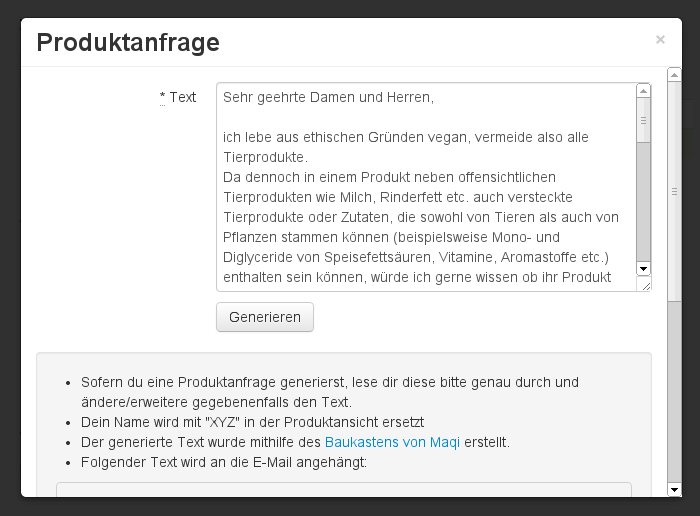
\includegraphics[scale=0.5]{pics/create_inquiry.png}
  \caption{Erstellung einer Produktanfrage mit generiertem Text}
  \label{img:create_inquiry}
\end{figure}

Innerhalb des Erstellungsfensters (zu sehen in 
Abbildung~\ref{img:create_inquiry}) befinden sich zusätzlich zu einem 
Eingabefeld, in dem eine Produktanfrage durch den "`Generieren"'-Button erstellt 
werden kann, noch Hinweise, den generierten Text falls notwendig zu ändern bzw. 
zu erweitern, welche Zutaten in dem Produkt potentiell
vegan sein könnten und woher der generierte Text stammt.
Ebenfalls dazu, ob der Name beim
Erstellen in der Produktübersicht anonymisiert wird (was in den 
Nutzer*ineinstellungen geändert werden kann)
sowie ein Text, der den*die Hersteller*in darauf hinweist, dass dies
eine automatisch generierte Anfrage ist, der Betreff daher nicht geändert
werden soll und die Antwort veröffentlicht wird.\\
Der Betreff soll dem System bei einer Antwort von einem*einer Hersteller*in 
ermöglichen, diese automatisch anhand der im Betreff befindlichen ID des 
Produktes, also einer Nummer in der Datenbank, zu erkennen und unterhalb des 
betreffenden Produktes zu speichern. Dies funktioniert allerdings nur, wenn ein 
Mailserver auf dem System, auf dem \name läuft, eingerichtet ist und diese 
Mails an \name übergibt. Zudem wird diese Antwort noch nicht direkt auf der 
Produktübersicht angezeigt, sie muss zuerst von dem*der Ersteller*in 
überprüft werden und die Veganität eingestellt werden.\\
Existiert kein Mailserver, der die E-Mails annehmen kann, kann eine Antwort, da 
sie auch durch den gesetzten Reply-To-Header in der E-Mail an den*die Nutzer*in 
geschickt werden soll, von diesem*dieser in der Nutzer*inübersicht erstellt 
werden, was in Abbildung~\ref{img:create_inquiry_2} zu sehen ist.

\begin{figure}[ht]
  \centering
  
\includegraphics[scale=0.5]{pics/create_inquiry_2.png}
  \caption{Erstellungsmöglichkeit einer Antwort auf eine Produktanfrage in der 
Übersicht von einem*einer Nutzer*in}
  \label{img:create_inquiry_2}
\end{figure}

Die Veganität der Produktanfragen (hier: \code{inquiries}), welche zur
Berechnung der Veganität eines Produktes benutzt wird, berechnet sich wie in 
Algorithmus~\ref{algo:veganity_inquiries} dargestellt. Ist weder eine Quelle 
noch eine Produktanfrage vorhanden, ist die Veganität unbekannt 
(Zeile~\ref{algo:veganity_inquiries:1}), ist nur eine Quelle vorhanden, 
entspricht diese auch der Produktanfragen-Veganität 
(Zeile~\ref{algo:veganity_inquiries:2}) und ansonsten ist die 
Produktanfragen-Veganität die Veganität der letzten Produktanfrage bzw. der 
Antwort darauf (Zeile~\ref{algo:veganity_inquiries:3}).\\
Die Quelle, die im Algorithmus genutzt 
wird (hier: \code{source}), kann bei der Erstellung eines Produktes mit den 
entsprechenden Rechten (siehe Abschnitt~\ref{sec:implementation:gamification}) 
angegeben werden und entspricht
der ersten Antwort auf eine nicht existente Produktanfrage. Diese Quelle 
kann ein Link zu einer schon
vorhandenen Produktanfrage (mit Antwort) sein, die z.\,B. auf einem Blog 
oder in einem
Forum vorhanden ist oder ein Link zu der Seite von einem*einer Hersteller*in, 
in dem auf die Veganität des Produktes eingegangen wird.

\begin{algorithm}[ht]
  \SetAlgoLined
  \KwIn{All inquiries and the source associated with a product}
  \KwOut{Veganity of the inquiries (including the source)}
  \BlankLine
  
  \uIf{source is empty and inquiries are empty}{
    \Return UNKNOWN\label{algo:veganity_inquiries:1}
  } \uElseIf{source is not empty and inquiries are empty}{
    \Return veganity of the source\label{algo:veganity_inquiries:2}
  } \Else{
    \Return veganity of the last inquiry\label{algo:veganity_inquiries:3}
  }
  \caption{Berechnung der Produktanfragen-Veganität eines Produktes}
  \label{algo:veganity_inquiries}
\end{algorithm}

\subsection{Kommentarerstellung und Veganitätsbestimmung}
\label{sec:implementation:comments}

Wie in Abschnitt~\ref{sec:concept:comments} beschrieben wurde, können 
Kommentare von angemeldeten Nutzer*innen erstellt werden und können auch in die 
Berechnung der Veganität mit einfließen, da zu jedem Kommentar eine Veganität 
ausgewählt werden muss, was in Abbildung~\ref{img:create_comment} dargestellt 
ist.

\begin{figure}[ht]
  \centering
  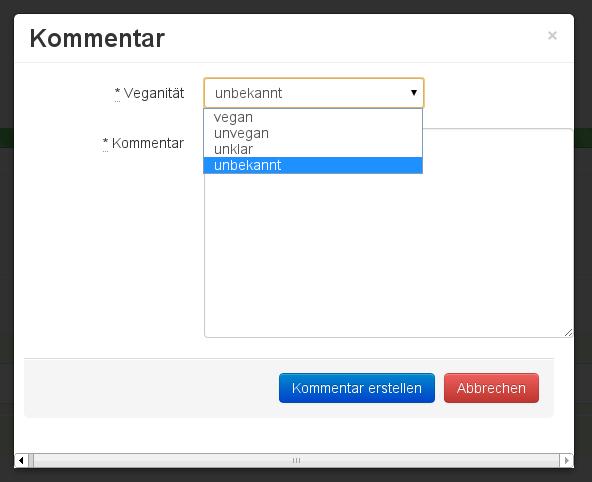
\includegraphics[scale=0.5]{pics/create_comment.png}
  \caption{Kommentar erstellen}
  \label{img:create_comment}
\end{figure}

Die Kommentare werden unterhalb eines Produktes je nach Veganität mit einer 
anderen Farbe und einem anderen Symbol angezeigt und können auch dort erstellt 
werden, wie in Abbildung~\ref{img:comments} zu sehen ist.

\begin{figure}[ht]
  \centering
  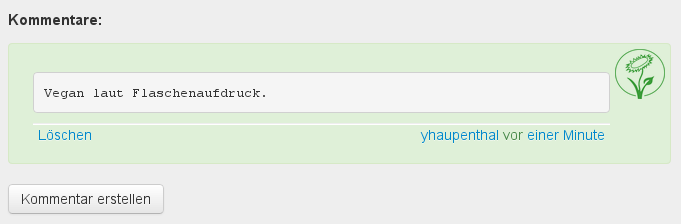
\includegraphics[scale=0.5]{pics/comments.png}
  \caption{Kommentare}
  \label{img:comments}
\end{figure}

Die Berechnung der Veganität aller Kommentare zu einem Produkt ist in 
Algorithmus~\ref{algo:veganity_comments} beschrieben.

\begin{algorithm}[ht]
  \SetAlgoLined
  \KwIn{All comments associated with a product}
  \KwOut{Veganity of these comments}
  \BlankLine
  
  \uIf{there is no comment}{
    \Return UNKNOWN\;
  }\Else{
    \Return veganity of last comment\;
  }

  \caption{Berechnung der Kommentar-Veganität eines Produktes}
  \label{algo:veganity_comments}
\end{algorithm}

Sind keine Kommentare vorhanden, ist die Kommentar-Veganität unbekannt (Zeile 
2), ansonsten wird sie durch den letzten Kommentar festgelegt (Zeile 4).

\subsection{Ermittlung der Produkt-Veganität}
\label{sec:implementation:veganity-2}
\label{sec:implementation:veganity}
\label{sec:implementation:product}

Die Produkt-Veganität wird dynamisch
aus den vorhandenen Zutaten, Produktanfragen und Kommentaren
berechnet. Der zugrunde liegende Algorithmus (\ref{algo:veganity_product}) wird 
im Folgenden beschrieben.

\begin{algorithm}[ht]
  \SetAlgoLined
  \KwIn{A product and its underlying ingredients, comments and inquiries}
  \KwOut{The veganity of this product}

  \BlankLine
 
  define set\label{algo:veganity_product:1}\;
  \uIf{ingredients are empty}{
    set = \{UNKNOWN, veganity of the inquiries, 
    veganity of the comments\}\;
  }\uElseIf{there is one ingredient and it's fixed}{
    set = \{veganity of the ingredients, 
    veganity of the inquiries, 
    veganity of the comments\}\;
  }\uElseIf{there is one ingredient and it's not 
fixed}{\label{algo:veganity_product:7}
    set = \{veganity of the inquiries, 
veganity of the comments\}\;\label{algo:veganity_product:8}
  }\Else{
    set = \{veganity of the ingredients, 
    veganity of the inquiries, 
    veganity of the comments\}\;
  }\label{algo:veganity_product:2}
  
  \BlankLine
 
  \If{size of set is bigger than 2 and (veganity of the inquiries or 
of the comments is VEGAN) and veganity of the ingredients is not 
NOT\_VEGAN}{\label{algo:veganity_product:3}
    set = \{veganity of the inquiries, 
    veganity of the comments\}\;
  }\label{algo:veganity_product:4}

  \BlankLine
 
  \uIf{set contains NOT\_VEGAN}{\label{algo:veganity_product:5}
    \Return NOT\_VEGAN\;
  }\uElseIf{set contains UNCERTAIN}{
    \Return UNCERTAIN\;
  }\uElseIf{set contains VEGAN}{
    \Return VEGAN\;
  }\Else{
    \Return UNKNOWN\;
  }\label{algo:veganity_product:6}
 
  \caption{Berechnung der Veganität eines Produktes}
  \label{algo:veganity_product}
\end{algorithm}

Es werden zunächst die anderen Veganitäten (Zutaten, Produktanfragen und 
Kommentare) berechnet und in einer Menge gespeichert 
(Zeilen~\ref{algo:veganity_product:1}\,--\,\ref{algo:veganity_product:2}). In 
den Zeilen~\ref{algo:veganity_product:7} und \ref{algo:veganity_product:8} wird 
ersichtlich, wie die Produkt-Veganität einer Zutat (siehe 
Abschnitt~\ref{sec:implementation:ingredients} berechnet wird, nämlich nur 
durch die Produktanfragen und Kommentare.\\
Im Fall, dass ein Produkt keine unveganen aber z.\,B. unklare Zutaten enthält, 
die Produkt\-anfragen- oder Kommentar-Veganität aber vegan ist, muss die 
Veganität gewichtet werden, indem die Zutaten-Veganität ignoriert wird 
(Zeilen~\ref{algo:veganity_product:3}\,--\,\ref{algo:veganity_product:4}).
Anschließend wird die Produkt-Veganität mittels einer Fallunterscheidung 
bestimmt 
(Zeilen~\ref{algo:veganity_product:5}\,--\,\ref{algo:veganity_product:6}).

Allerdings wurde durch eine Worst-Case-Laufzeit von $\mathcal{O}
(n^k)$, die theoretisch bei einem Update einer Zutaten-Veganität und einem
damit verbundenen Update aller Produkte auftreten würde,
die Berechnung der Veganität teilweise ausgelagert.
Die Aktualität wird dabei durch ein Programm gewährleistet, das
die Veganitäten der Produkte und Zutaten aktualisiert und stündlich ausgeführt 
wird.
Zudem wird die
jeweilige Veganität beim Anklicken der Übersichtsseite eines Produktes
oder einer Zutat auf den neuesten Stand gebracht, sodass die
Aktualität für den*die Nutzer*in immer gegeben ist.

\subsection{Internationalisierung/Lokalisierung}
\label{sec:implementation:i18n}
\label{sec:implementation:l10n}

Durch die Internationalisierung, d.\,h.
die Gestaltung eines Systems, welches leicht an verschiedene Sprachen bzw. 
Kulturen angepasst werden kann, die auch in \name verwendet wurde, können 
leicht weitere Sprachen integriert werden. Dies geschieht durch die 
Lokalisierung,
d.\,h. das Übersetzen von 
Sprachdateien in verschiedene Sprachen.\\
Aktuell ist \name dabei in deutscher Sprache verfügbar, da 
sich diese Arbeit vorrangig an den deutschen Markt richtet.

\clearpage
\section{Integration in das \acl{IRL}}
\label{sec:implementation:irl}

Wie in Abschnitt~\ref{sec:concept:irl} beschrieben, sollte auch im \ac{IRL}
eine Instanz von \name als Demonstrator in Betrieb genommen werden.\\
Dabei wurde der gleiche Programmcode mit zwei Änderungen benutzt:

\begin{enumerate}
  \item Es wurden keine externen Dienstanbieter*innen zur Authentifizierung wie 
Google 
implementiert, da es nur
    ein*e Nutzer*in gibt. Die Webanwendung wurde mit
    "`Htaccess"' geschützt.
  \item Da diese Instanz nur ein Demonstrator ist, wurden keine
    echten E-Mailadressen benutzt, stattdessen gehen alle
    ausgehenden E-Mails an die selbe Adresse.
\end{enumerate}

Als Datengrundlage wurde ein Speicherauszug aus der Datenbank (Dump) von 
\name nach einer ein-monatigen Beta-Phase
verwendet.
Zusätzlich zur Webanwendung gibt es auch im \ac{IRL} eine Instanz der
mobilen App, hier wurde lediglich die \ac{URL}, von der die Daten
kommen, ausgetauscht.

\section{Technische Dokumentation}
\label{sec:implementation:docu}

Die technische Dokumentation in englischer Sprache befindet sich auf der beigelegten CD im
Verzeichnis \code{yava/doc}. Die sich dort befindliche
Datei \code{index.html} kann in einem Browser geöffnet werden
und enthält die technischen Schritte die zur Installation von \name
mit allen Komponenten auf einem GNU/Linux-Betriebssystem benötigt
werden. Daneben befinden sich dort alle mit Kommentaren versehenen Klassen und
Module sowie die jeweiligen Methoden.\\
Zusätzlich befindet sich die Dokumentation auf GitHub
\citeweb{github:tohn}.

\section{Lizenzen}
\label{sec:licenses}
\label{sec:implementation:licenses}
Dadurch, dass alle, die eine (vegane) Produktdatenbank erstellen
wollen, jedes Mal von neuem beginnen müssen weil die existierenden
Datenbanken selten eine Möglichkeit haben, alle Daten herunterzuladen,
soll dies ein Versuch sein, eine komplett freie Datenbank zu erstellen.
Deshalb werden alle Daten der Datenbank -- exklusive die Daten der
Nutzer*innen -- unter der CC0-Lizenz veröffentlicht \citeweb{cc:cc0}
und als kompletter Speicherauszug der Datenbank erhältlich sein
\citeweb{yh:dump}.\\
Dies wird gewährleistet durch ein Programm, das
täglich um Mitternacht ein Skript ausführt, welches aus der Datenbank die
nötigen Tabellen extrahiert und in Dateien speichert.
Diese Dateien sind online verfügbar und werden mit Hilfe des
Webservers, in diesem Fall \code{lighttpd}, angezeigt, wie in
Abbildung~\ref{image:dump} zu sehen ist.

\begin{figure}[ht]
  \centerline{
    \frame{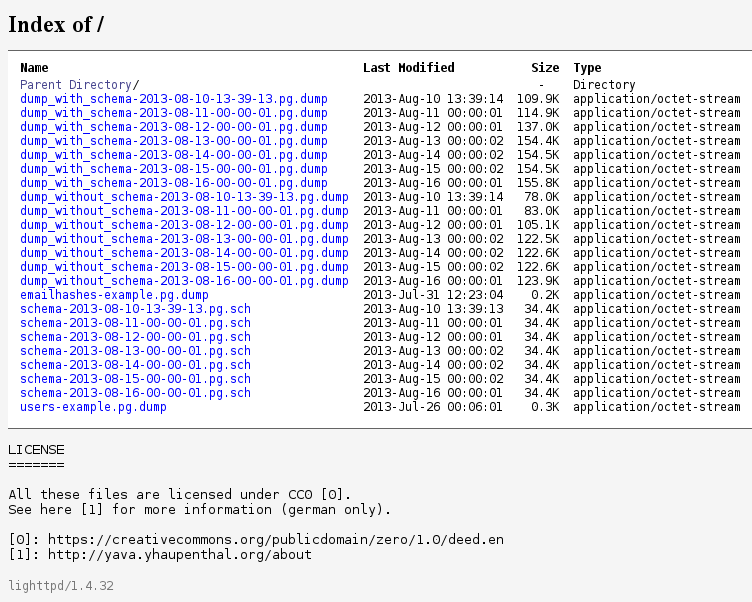
\includegraphics[scale=0.5]{pics/dump.png}}
  }
  \caption{Dump der Datenbank, dargestellt durch den Webserver}
  \label{image:dump}
\end{figure}

Das dazu notwendige Skript sowie das ausführende Programm befinden sich 
ebenfalls in
der technischen Dokumentation, siehe dazu 
Abschnitt~\ref{sec:implementation:docu}.

Der Programmcode der Website und der mobilen Anwendung (App) sind unter der 
Lizenz "`GPLv3"' verfügbar \citeweb{gplv3}, da alle
Weiterentwicklungen wieder in die ursprüngliche Arbeit einfließen
sollen.

Der Code dieser Arbeit, sämtliche vorherigen Dokumente und der
Programmcode für Website und App sind auf GitHub, einer
Plattform für Software-Entwicklungsprojekte erhältlich
\citeweb{github:tohn}.

Der Code der Arbeit selbst und sämtliche vorherigen Dokumente sind unter der 
CC0-Lizenz erhältlich \citeweb{cc:cc0}.